\documentclass[12pt]{article}
\usepackage[T1,T2A]{fontenc}
\usepackage[utf8]{inputenc}
\usepackage{graphicx}
\usepackage[english, russian]{babel}
\usepackage[colorlinks=true, 
linkcolor=blue,
filecolor=blue,
citecolor=blue, 
urlcolor=blue,
unicode=true]{hyperref} 
\usepackage{mathtools}
\usepackage{amsmath,amssymb,amsthm,latexsym}
\usepackage{mathtext}
\usepackage{multirow}
\usepackage{indentfirst}
\usepackage{enumerate}
\usepackage{verbatim}
\usepackage{bigstrut}
\usepackage{booktabs}
\usepackage[left=12mm, top=10mm, right=15mm, bottom=15mm, nohead, footskip=10mm]{geometry}
\usepackage{wrapfig}
\usepackage{array}
\usepackage[rightcaption]{sidecap}
\usepackage{color,colortbl}

\usepackage{listings} % Для вставки кода
\usepackage{xcolor}   % Цвета для кода
\usepackage{float}    % Плавающие объекты

% --- Авторская настройка для адекватной вставки кода с использованием кириллицы ---
\lstdefinestyle{mypython}{
    language=Python,
    basicstyle=\ttfamily\scriptsize,
    keywordstyle=\color{blue}\bfseries,
    stringstyle=\color{red},
    commentstyle=\color{green!60!black},
    numbers=left,
    numberstyle=\tiny\color{gray},
    stepnumber=1,
    numbersep=8pt,
    showspaces=false,
    showstringspaces=false,
    tabsize=4,
    frame=single,
    rulecolor=\color{black},
    breaklines=true,
    breakatwhitespace=false,
    captionpos=b,
    xleftmargin=15pt,
    xrightmargin=5pt,
    framexleftmargin=12pt,
    backgroundcolor=\color{gray!5},
    literate=%
        {а}{{\cyra}}1 {б}{{\cyrb}}1 {в}{{\cyrv}}1 {г}{{\cyrg}}1 {д}{{\cyrd}}1
        {е}{{\cyre}}1 {ё}{{\cyrie}}1 {ж}{{\cyrzh}}1 {з}{{\cyrz}}1 {и}{{\cyri}}1
        {й}{{\cyrishrt}}1 {к}{{\cyrk}}1 {л}{{\cyrl}}1 {м}{{\cyrm}}1 {н}{{\cyrn}}1
        {о}{{\cyro}}1 {п}{{\cyrp}}1 {р}{{\cyrr}}1 {с}{{\cyrs}}1 {т}{{\cyrt}}1
        {у}{{\cyru}}1 {ф}{{\cyrf}}1 {х}{{\cyrh}}1 {ц}{{\cyrc}}1 {ч}{{\cyrch}}1
        {ш}{{\cyrsh}}1 {щ}{{\cyrshch}}1 {ъ}{{\cyrhrdsn}}1 {ы}{{\cyrery}}1
        {ь}{{\cyrsftsn}}1 {э}{{\cyrerev}}1 {ю}{{\cyryu}}1 {я}{{\cyrya}}1
        {А}{{\CYRA}}1 {Б}{{\CYRB}}1 {В}{{\CYRV}}1 {Г}{{\CYRG}}1 {Д}{{\CYRD}}1
        {Е}{{\CYRE}}1 {Ё}{{\CYRIE}}1 {Ж}{{\CYRZH}}1 {З}{{\CYRZ}}1 {И}{{\CYRI}}1
        {Й}{{\CYRISHRT}}1 {К}{{\CYRK}}1 {Л}{{\CYRL}}1 {М}{{\CYRM}}1 {Н}{{\CYRN}}1
        {О}{{\CYRO}}1 {П}{{\CYRP}}1 {Р}{{\CYRR}}1 {С}{{\CYRS}}1 {Т}{{\CYRT}}1
        {У}{{\CYRU}}1 {Ф}{{\CYRF}}1 {Х}{{\CYRH}}1 {Ц}{{\CYRC}}1 {Ч}{{\CYRCH}}1
        {Ш}{{\CYRSH}}1 {Щ}{{\CYRSHCH}}1 {Ъ}{{\CYRHRDSN}}1 {Ы}{{\CYRERY}}1
        {Ь}{{\CYRSFTSN}}1 {Э}{{\CYREREV}}1 {Ю}{{\CYRYU}}1 {Я}{{\CYRYA}}1
}
\lstset{style=mypython}

\definecolor{darkishgreen}{RGB}{39,203,22}
\definecolor{LightCyan}{rgb}{0.88,1,1}
\definecolor{Gray}{gray}{0.8}

\author{Михайлов П., Гришин А., Ткачёв Д.}
\title{Рабочий протокол и отчет по лабораторной работе № 3.05\\}
\date{\today}

\begin{document}

% ====================== ТИТУЛЬНЫЙ ЛИСТ ======================
\begin{titlepage}
    \centering
    % Шапка
    {\fontsize{11}{13}\selectfont \textbf{Министерство науки и высшего образования Российской Федерации}} \\
    {\fontsize{7}{10}\selectfont ФЕДЕРАЛЬНОЕ ГОСУДАРСТВЕННОЕ АВТОНОМНОЕ ОБРАЗОВАТЕЛЬНОЕ УЧРЕЖДЕНИЕ ВЫСШЕГО ОБРАЗОВАНИЯ} \\
    \vspace{0.2cm} 
    {\fontsize{14}{17}\selectfont \textbf{«НАЦИОНАЛЬНЫЙ ИССЛЕДОВАТЕЛЬСКИЙ УНИВЕРСИТЕТ ИТМО»}}
    
    \vspace{1cm} 
    
    % Информация о группе
    {\fontsize{12}{14}\selectfont \textbf{Группа ФИЗ ПИИКТ 2.4.1}}
    
    \vspace{1cm}
    
    % Информация о дисциплине
    {\fontsize{12}{14}\selectfont \textbf{Дисциплина: Физика}}
    
    \vspace*{\fill}
    
    % Заголовок работы
    {\fontsize{18}{22}\selectfont \textbf{ЛАБОРАТОРНАЯ РАБОТА № 3.05}} \\
    \vspace{0.5cm}
    {\fontsize{14}{17}\selectfont \textbf{по теме: «Температурная зависимость электрического сопротивления металла и полупроводника»}}
    
    \vspace{3cm}
    
    % Блок выполнил/проверил
    \begin{flushright}
        \fontsize{12}{14}\selectfont
        Выполнили: \\
        Михайлов Пётр Сергеевич\\
        Гришин Артём Евгеньевич\\
        Ткачев Денис Владимирович\\
        \vspace{1em}
        Проверил: \\
        Иванов Владимир Сергеевич
    \end{flushright}
    
    \vfill
    
    % Подвал
    {\fontsize{12}{14}\selectfont
    Санкт-Петербург, 2026
    }
\end{titlepage}

\setcounter{page}{2}

\newpage
% ====================== СОДЕРЖАНИЕ ======================
\tableofcontents
\newpage

\section{Цель работы}
1. Получить зависимость электрического сопротивления металлического и полупроводникового образцов в диапазоне температур от комнатной до $75~^{\circ}\text{C}$.\\

2. По результатам измерений вычислить температурный коэффициент сопротивления металла и ширину запрещенной зоны полупроводника.

\section{Задачи, решаемые при выполнении работы}
\begin{itemize}
    \item Экспериментально исследовать изменение силы тока и напряжения на металлическом и полупроводниковом образцах при нагреве и охлаждении.
    \item Рассчитать значения сопротивлений образцов для каждого температурного шага.
    \item Построить графики температурных зависимостей: $R(t)$ для металла и $\ln (R / 1\,\text{Ом})$ от обратной температуры $10^3/T$ для полупроводника.
    \item Методом разбиения экспериментальных данных на независимые пары рассчитать температурный коэффициент сопротивления металла $\alpha$ и ширину запрещенной зоны полупроводника $E_g$.
    \item Оценить полные погрешности измерений (совместно случайные и систематические приборные) и идентифицировать материалы образцов по справочным данным.
\end{itemize}

\section{Объект исследования и метод эксперимента}
Исследуются закономерности протекания электрического тока в средах с различными механизмами проводимости. В металлах концентрация свободных носителей заряда (электронов) практически неизменна, а сопротивление растет с ростом температуры за счет увеличения частоты столкновений с фононами (тепловыми колебаниями решетки). В собственных полупроводниках проводимость носит активационный характер: тепловая энергия приводит к разрыву ковалентных связей и генерации пар электрон-дырка, из-за чего концентрация носителей и проводимость экспоненциально растут с температурой, а сопротивление падает.

\section{Экспериментальная установка}
Экспериментальная установка включает в себя измерительный стенд «СЗ-ТТ01», содержащий теплоизолированную мини-печь с исследуемыми образцами (металлическим и полупроводниковым), электрический нагреватель и цифровой термодатчик. Питание измерительных цепей осуществляется от генератора постоянного напряжения ГН1. Регистрация значений силы тока $I$ и падения напряжения $U$ на образцах производится многофункциональным цифровым блоком амперметра-вольтметр АВ1. В цепь полупроводника последовательно включен балластный резистор $R_{\text{огр}} = 680~\text{Ом}$ для предотвращения токовой перегрузки при интенсивном нагреве образца.

\begin{figure}[H]
    \centering
    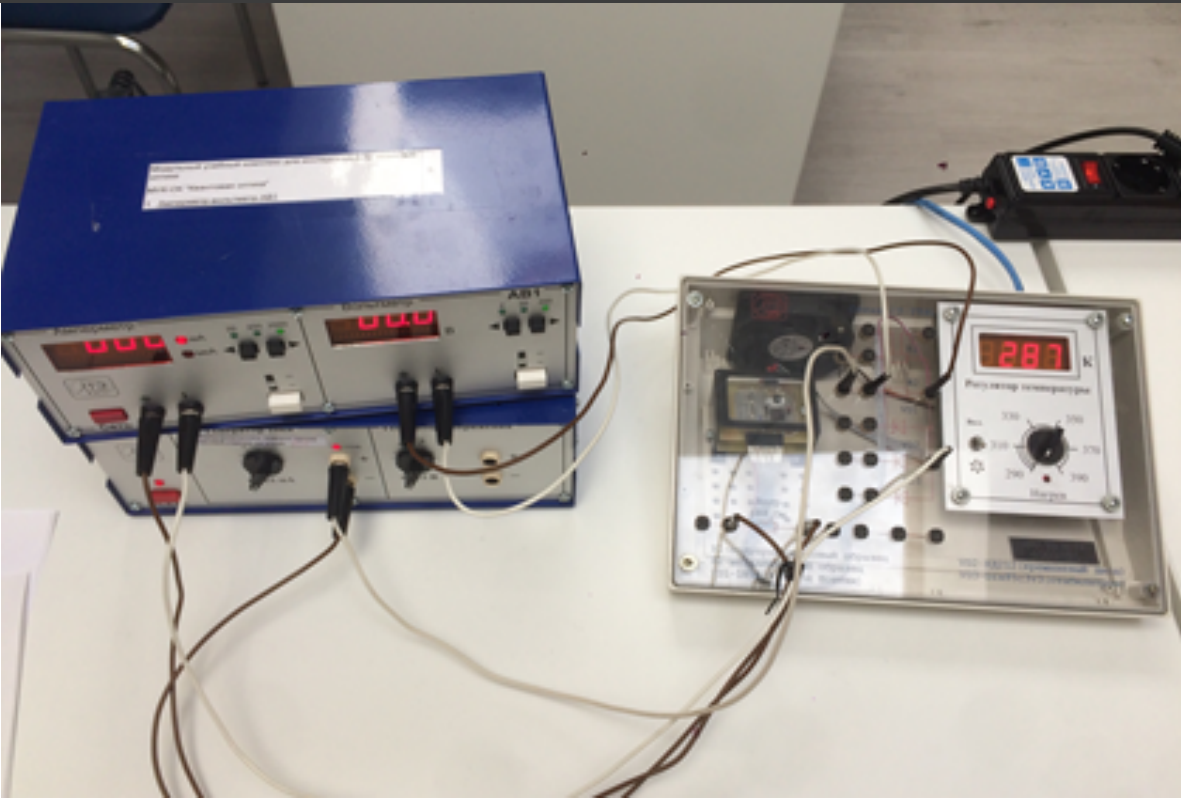
\includegraphics[width=0.9\textwidth]{Experimental_setup.png}
    \caption{Общий вид лабораторной установки}
    \label{fig:setup}
\end{figure}

\begin{figure}[H]
    \centering
    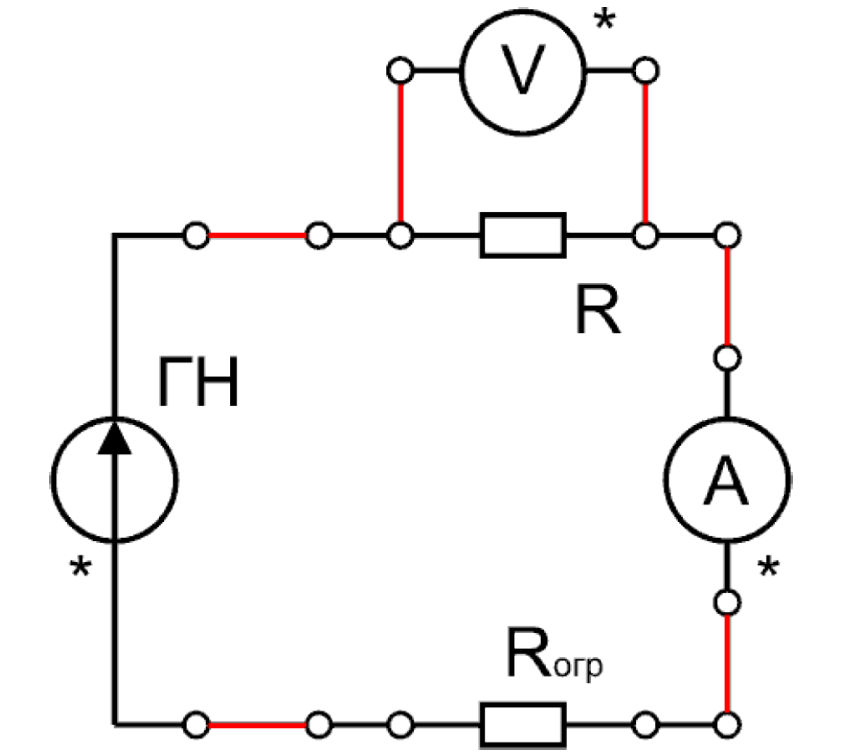
\includegraphics[width=0.65\textwidth]{circuit_diagram.png} 
    \caption{Принципиальная электрическая схема установки}
    \label{fig:circuit_diagram}
\end{figure}

В соответствии с техническим паспортом стенда, измерительные приборы обладают следующими метрологическими характеристиками:
\begin{itemize}
    \item Диапазон измерения вольтметра: $0{-}2~\text{В}$, разрешение (ЕДР) составляет $0{,}001~\text{В}$. Приборная погрешность: $\Delta U_{\text{приб}} = \pm(0{,}5\% \cdot U + 2 \cdot \text{ЕДР})$.
    \item Диапазон измерения амперметра: $0{-}2000~\text{мкА}$, разрешение (ЕДР) составляет $1~\text{мкА}$. Приборная погрешность: $\Delta I_{\text{приб}} = \pm(0{,}5\% \cdot I + 2 \cdot \text{ЕДР})$.
    \item Погрешность измерения температуры термодатчиком: $\Delta T_{\text{приб}} = \pm 0{,}5~\text{К}$.
\end{itemize}

\section{Рабочие формулы}
Сопротивление образца на каждом шаге определяется по закону Ома:
\begin{equation} \label{eq:ohm}
    R = \frac{U}{I}
\end{equation}

Линейная температурная зависимость сопротивления металла:
\begin{equation} \label{eq:metal_linear}
    R_M = R_0(1 + \alpha t)
\end{equation}
Рабочая формула метода пар для вычисления температурного коэффициента сопротивления металла $\alpha$:
\begin{equation} \label{eq:alpha_pairs}
    \alpha_{ij} = \frac{R_i - R_j}{R_j \cdot t_i - R_i \cdot t_j}
\end{equation}

Экспоненциальная зависимость сопротивления собственного полупроводника:
\begin{equation} \label{eq:semi_exponential}
    R_n = R_m \exp\left(\frac{E_g}{2kT}\right) \implies \ln(R_n / 1\,\text{Ом}) = \ln(R_m / 1\,\text{Ом}) + \frac{E_g}{2kT}
\end{equation}
Рабочая формула метода пар для оценки ширины запрещенной зоны полупроводника $E_g$:
\begin{equation} \label{eq:eg_pairs}
    E_{gij} = 2k \frac{\ln R_i - \ln R_j}{\frac{1}{T_i} - \frac{1}{T_j}} = 2k T_i T_j \frac{\ln(R_i / R_j)}{T_j - T_i}
\end{equation}
Где постоянная Больцмана $k = 1{,}380649 \cdot 10^{-23}~\text{Дж/К} \approx 8{,}61733 \cdot 10^{-5}~\text{эВ/К}$.

Полная абсолютная погрешность результатов косвенных измерений рассчитывается путем квадратичного суммирования случайной погрешности (оцененной по коэффициенту Стьюдента) и систематической приборной погрешности:
\begin{equation} \label{eq:total_error}
    \Delta_{\text{полн}} = \sqrt{\Delta_{\text{случ}}^2 + \Delta_{\text{приб}}^2}
\end{equation}

\section{Измерительные приборы}
\begin{table}[H]
\centering
\caption{Спецификация используемого оборудования и средств измерений}
\vspace{0.2cm}
\small
\begin{tabular}{cll}
\toprule
№ & Наименование & Назначение \\ 
\midrule
1 & Стенд «СЗ-ТТ01» & Содержит исследуемые образцы, нагреватель и термодатчик \\ 
2 & Генератор напряжения ГН1 & Источник питания постоянного тока для измерительной цепи \\ 
3 & Амперметр-вольтметр АВ1 & Измерение силы тока ($I$) и падения напряжения ($U$) на образцах \\
4 & Резистор $R_{\text{огр}} = 680~\text{Ом}$ & Ограничение тока в цепи полупроводника при сильном нагреве \\
\bottomrule
\end{tabular}
\end{table}

\newpage
\section{Результаты прямых измерений}

\subsection{Полупроводниковый образец}

\begin{figure}[H]
    \centering
    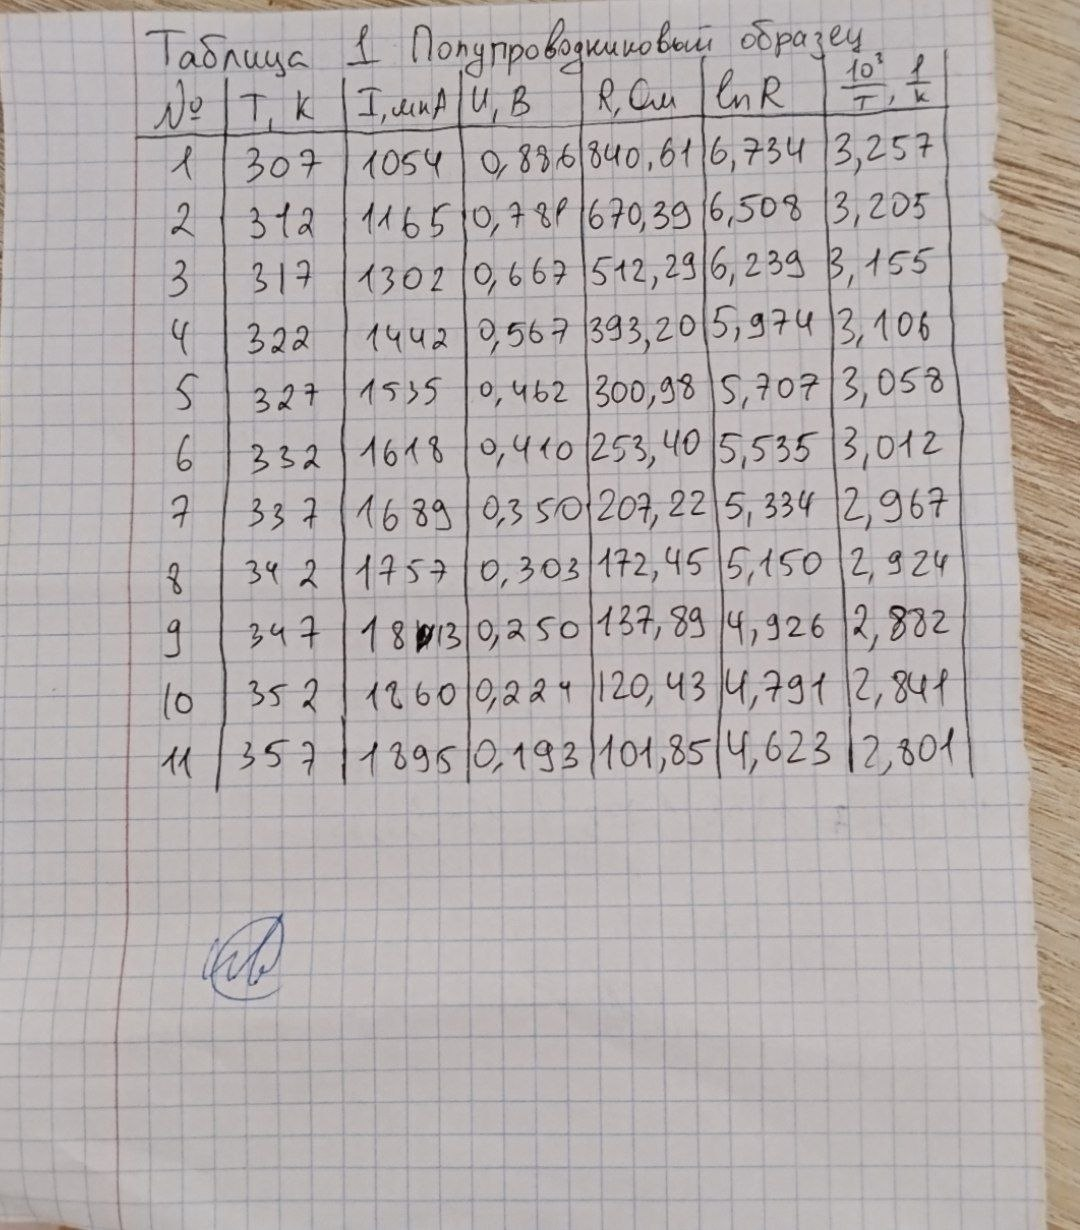
\includegraphics[width=0.64\textwidth]{handwritten_table1.jpg}
    \caption{Рукописный протокол измерений полупроводника}
\end{figure}

\begin{table}[H]
\centering
\caption{Экспериментальные данные прямых измерений полупроводникового образца}
\vspace{0.2cm}
\small
\begin{tabular}{ccccccc}
\toprule
№ & $T$, К & $I$, мкА & $U$, В & $R$, Ом & $\ln (R / 1\,\text{Ом})^*$ & $\frac{10^3}{T}$, К$^{-1}$ \\
\midrule
1  & 307 & 1054 & 0.886 & 840.61 & 6.734 & 3.257 \\
2  & 312 & 1165 & 0.781 & 670.39 & 6.508 & 3.205 \\
3  & 317 & 1302 & 0.667 & 512.29 & 6.239 & 3.155 \\
4  & 322 & 1442 & 0.567 & 393.20 & 5.974 & 3.106 \\
5  & 327 & 1535 & 0.462 & 300.98 & 5.707 & 3.058 \\
6  & 332 & 1618 & 0.410 & 253.40 & 5.535 & 3.012 \\
7  & 337 & 1689 & 0.350 & 207.22 & 5.334 & 2.967 \\
8  & 342 & 1757 & 0.303 & 172.45 & 5.150 & 2.924 \\
9  & 347 & 1813 & 0.250 & 137.89 & 4.926 & 2.882 \\
10 & 352 & 1860 & 0.224 & 120.43 & 4.791 & 2.841 \\
11 & 357 & 1895 & 0.193 & 101.85 & 4.623 & 2.801 \\
\bottomrule
\end{tabular}
\par\vspace{0.12cm}
\raggedright \footnotesize $^*$ Логарифм берется от безразмерного численного значения сопротивления.
\end{table}

\newpage
\subsection{Металлический образец}

\begin{figure}[H]
    \centering
    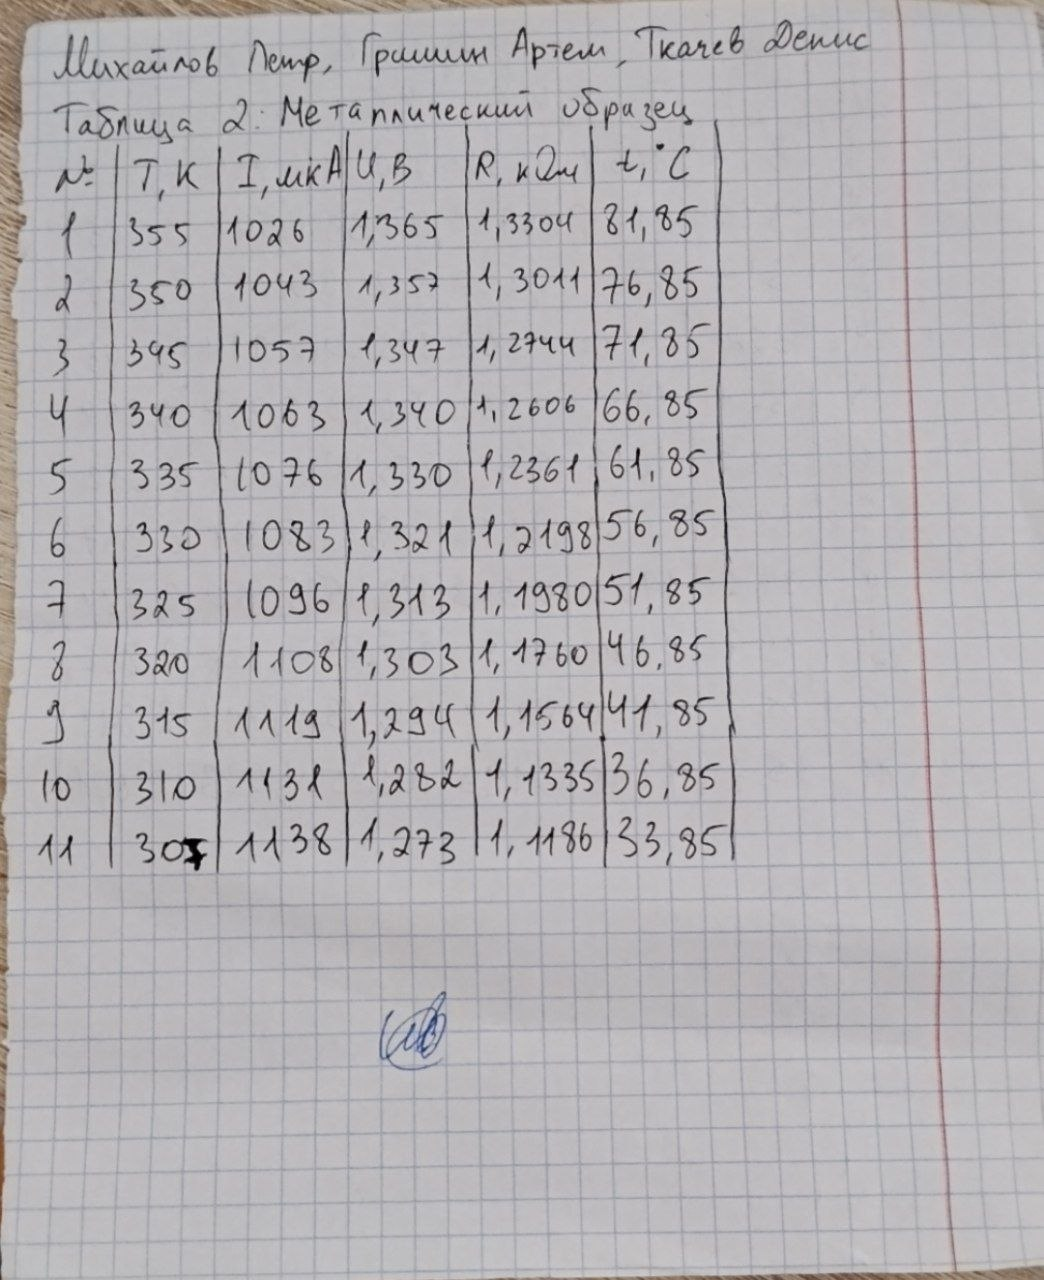
\includegraphics[width=0.65\textwidth]{handwritten_table2.jpg}
    \caption{Рукописный протокол измерений металла}
\end{figure}

\begin{table}[H]
\centering
\caption{Экспериментальные данные прямых измерений металлического образца}
\vspace{0.2cm}
\small
\begin{tabular}{cccccc}
\toprule
№ & $T$, К & $I$, мкА & $U$, В & $R$, кОм & $t$, $^{\circ}\text{C}$ \\
\midrule
1  & 355 & 1026 & 1.365 & 1.3304 & 81.85 \\
2  & 350 & 1043 & 1.357 & 1.3011 & 76.85 \\
3  & 345 & 1057 & 1.347 & 1.2744 & 71.85 \\
4  & 340 & 1063 & 1.340 & 1.2606 & 66.85 \\
5  & 335 & 1076 & 1.330 & 1.2361 & 61.85 \\
6  & 330 & 1083 & 1.321 & 1.2198 & 56.85 \\
7  & 325 & 1096 & 1.313 & 1.1980 & 51.85 \\
8  & 320 & 1108 & 1.303 & 1.1760 & 46.85 \\
9  & 315 & 1119 & 1.294 & 1.1564 & 41.85 \\
10 & 310 & 1131 & 1.282 & 1.1335 & 36.85 \\
11 & 307 & 1138 & 1.273 & 1.1186 & 33.85 \\
\bottomrule
\end{tabular}
\end{table}

\newpage
\section{Расчет результатов косвенных измерений}

\subsection{Обработка данных металлического образца}
Расчет значений сопротивления и пересчет температуры в шкалу Цельсия выполняется автоматически измерительным скриптом на основе закона Ома \eqref{eq:ohm}. 

\subsubsection*{Пример расчета для точки №1 (металлический образец):}
\begin{itemize}
    \item Сопротивление образца $R_M$:
    \begin{equation}
        R_{M1} = \frac{U_1}{I_1} = \frac{1{,}365~\text{В}}{1026 \cdot 10^{-6}~\text{А}} \approx 1330{,}41~\text{Ом} \approx 1{,}3304~\text{кОм}
    \end{equation}
    \item Температура по шкале Цельсия $t$:
    \begin{equation}
        t_1 = T_1 - 273{,}15 = 355 - 273{,}15 = 81{,}85~^{\circ}\text{C}
    \end{equation}
\end{itemize}

Для определения температурного коэффициента сопротивления металлический макромассив разбивается на независимые пары точек (1–6, 2–7, 3–8, 4–9, 5–10). Расчет коэффициентов $\alpha_{ij}$ проводится по формуле \eqref{eq:alpha_pairs}. Результаты расчета по парам сведены в таблицу \ref{tab:metal_pairs}.

\begin{table}[H]
\centering
\caption{Расчет температурного коэффициента сопротивления металла методом пар}
\label{tab:metal_pairs}
\vspace{0.2cm}
\small
\begin{tabular}{ccccc}
\toprule
Пара $i$--$j$ & $t_i, ~^{\circ}\text{C}$ & $t_j, ~^{\circ}\text{C}$ & $\Delta t, ~^{\circ}\text{C}$ & $\alpha_{ij} \cdot 10^{-3}, ~\text{К}^{-1}$ \\
\midrule
1--6  & 81.85 & 56.85 & 25.00 & 4.57 \\
2--7  & 76.85 & 51.85 & 25.00 & 4.19 \\
3--8  & 71.85 & 46.85 & 25.00 & 3.97 \\
4--9  & 66.85 & 41.85 & 25.00 & 4.25 \\
5--10 & 61.85 & 36.85 & 25.00 & 4.18 \\
\bottomrule
\end{tabular}
\end{table}

Среднее значение коэффициента составляет:
$$ \langle \alpha \rangle = 4{,}23 \cdot 10^{-3}~\text{К}^{-1} $$

\subsection{Обработка данных полупроводникового образца}
Логарифмирование численных значений сопротивлений и расчет величин $10^3/T$ проводятся на основе закона Ома \eqref{eq:ohm}.

\subsubsection*{Пример расчета для точки №1 (полупроводниковый образец):}
\begin{itemize}
    \item Сопротивление образца $R$:
    \begin{equation}
        R_1 = \frac{U_1}{I_1} = \frac{0{,}886~\text{В}}{1054 \cdot 10^{-6}~\text{А}} \approx 840{,}61~\text{Ом}
    \end{equation}
    \item Натуральный логарифм численного значения сопротивления:
    \begin{equation}
        \ln (R_1 / 1\,\text{Ом}) = \ln(840{,}61) \approx 6{,}734
    \end{equation}
    \item Обратная температура $\frac{10^3}{T}$:
    \begin{equation}
        \frac{10^3}{T_1} = \frac{1000}{307~\text{К}} \approx 3{,}257~\text{К}^{-1}
    \end{equation}
\end{itemize}

Для вычисления энергии активации (ширины запрещенной зоны) $E_g$ аналитическим методом данные разбиваются на независимые пары. Расчет выполняется по рабочей формуле \eqref{eq:eg_pairs}. Результаты попарного анализа представлены в таблице \ref{tab:semi_pairs}.

\begin{table}[H]
\centering
\caption{Расчет ширины запрещенной зоны полупроводника методом пар}
\label{tab:semi_pairs}
\vspace{0.2cm}
\small
\begin{tabular}{ccccc}
\toprule
Пара $i$--$j$ & $T_i, ~\text{К}$ & $T_j, ~\text{К}$ & $E_{gij}, ~\text{эВ}$ & $E_{gij} \cdot 10^{-19}, ~\text{Дж}$ \\
\midrule
1--6  & 307 & 332 & 0.842 & 1.349 \\
2--7  & 312 & 337 & 0.851 & 1.363 \\
3--8  & 317 & 342 & 0.814 & 1.304 \\
4--9  & 322 & 347 & 0.807 & 1.293 \\
5--10 & 327 & 352 & 0.727 & 1.165 \\
\bottomrule
\end{tabular}
\end{table}

Среднее значение ширины запрещенной зоны составляет:
$$ \langle E_g \rangle = 0{,}81~\text{эВ} = 1{,}30 \cdot 10^{-19}~\text{Дж} $$

\textit{Примечание:} Альтернативным графическим методом ширина запрещенной зоны может быть определена через тангенс угла наклона аппроксимирующей прямой линеаризованной зависимости $\ln (R / 1\,\text{Ом})$ от обратной температуры, физический смысл которой заложен в уравнении \eqref{eq:semi_exponential}.

\section{Расчет погрешностей измерений}
Для оценки случайных погрешностей результатов косвенных измерений использовалось распределение Стьюдента. Число независимых пар измерений $n = 5$, следовательно, число степеней свободы $\nu = n - 1 = 4$. Для доверительной вероятности $P = 0{,}95$ коэффициент Стьюдента составляет $t_{0{,}95; 4} = 2{,}78$.

Систематическая приборная составляющая абсолютной погрешности для косвенных величин, вычисленная методом переноса инструментальных неопределенностей измерительного стенда АВ1, составляет: $\Delta \alpha_{\text{приб}} \approx 0{,}05 \cdot 10^{-3}~\text{К}^{-1}$, $\Delta E_{g,\text{приб}} \approx 0{,}02~\text{эВ}$ ($0{,}03 \cdot 10^{-19}~\text{Дж}$).

\subsection{Погрешность коэффициента \texorpdfstring{$\alpha$}{alpha} металла}
Среднеквадратичное отклонение среднего значения $\langle \alpha \rangle$ рассчитывается как:
$$ S_{\langle \alpha \rangle} = \sqrt{\frac{\sum (\alpha_{ij} - \langle \alpha \rangle)^2}{n(n-1)}} \approx 0{,}097 \cdot 10^{-3}~\text{К}^{-1} $$
Случайная погрешность:
$$ \Delta \alpha_{\text{случ}} = t_{0{,}95; 4} \cdot S_{\langle \alpha \rangle} = 2{,}78 \cdot 0{,}097 \cdot 10^{-3} \approx 0{,}27 \cdot 10^{-3}~\text{К}^{-1} $$
Полная абсолютная погрешность с учетом приборной составляющей по формуле \eqref{eq:total_error}:
$$ \Delta \alpha = \sqrt{\Delta \alpha_{\text{случ}}^2 + \Delta \alpha_{\text{приб}}^2} = \sqrt{(0{,}27)^2 + (0{,}05)^2} \cdot 10^{-3} \approx 0{,}27 \cdot 10^{-3}~\text{К}^{-1} $$
Относительная погрешность измерений:
$$ \varepsilon_{\alpha} = \frac{\Delta \alpha}{\langle \alpha \rangle} \cdot 100\% = \frac{0{,}27 \cdot 10^{-3}}{4{,}23 \cdot 10^{-3}} \cdot 100\% \approx 6{,}4\% $$

Итоговый результат для температурного коэффициента металла:
\begin{equation}
    \alpha = (4{,}23 \pm 0{,}27) \cdot 10^{-3}~\text{К}^{-1} \quad (P = 0{,}95)
\end{equation}

\subsection{Погрешность ширины запрещенной зоны \texorpdfstring{$E_g$}{Eg} полупроводника}
Среднеквадратичное отклонение среднего значения $\langle E_g \rangle$:
$$ S_{\langle E_g \rangle} = \sqrt{\frac{\sum (E_{gij} - \langle E_g \rangle)^2}{n(n-1)}} \approx 0{,}022~\text{эВ} $$
Случайная погрешность:
$$ \Delta E_{g,\text{случ}} = t_{0{,}95; 4} \cdot S_{\langle E_g \rangle} = 2{,}78 \cdot 0{,}022 \approx 0{,}061~\text{эВ} $$
Полная абсолютная погрешность с учетом приборной составляющей по формуле \eqref{eq:total_error}:
$$ \Delta E_g = \sqrt{\Delta E_{g,\text{случ}}^2 + \Delta E_{g,\text{приб}}^2} = \sqrt{(0{,}061)^2 + (0{,}020)^2} \approx 0{,}06~\text{эВ} \approx 0{,}10 \cdot 10^{-19}~\text{Дж} $$
Относительная погрешность измерений:
$$ \varepsilon_{E_g} = \frac{\Delta E_g}{\langle E_g \rangle} \cdot 100\% = \frac{0{,}06}{0{,}81} \cdot 100\% \approx 7{,}4\% $$

Итоговый результат для ширины запрещенной зоны полупроводника:
\begin{align}
    E_g &= 0{,}81 \pm 0{,}06~\text{эВ} \quad (P = 0{,}95) \\
    E_g &= (1{,}30 \pm 0{,}10) \cdot 10^{-19}~\text{Дж} \quad (P = 0{,}95)
\end{align}

\newpage
\section{Визуализация данных}
Температурные зависимости для обоих исследуемых образцов построены с помощью разработанного скрипта на языке Python (полный компилируемый исходный код программы приведен в Приложении А).

\begin{figure}[H]
    \centering
    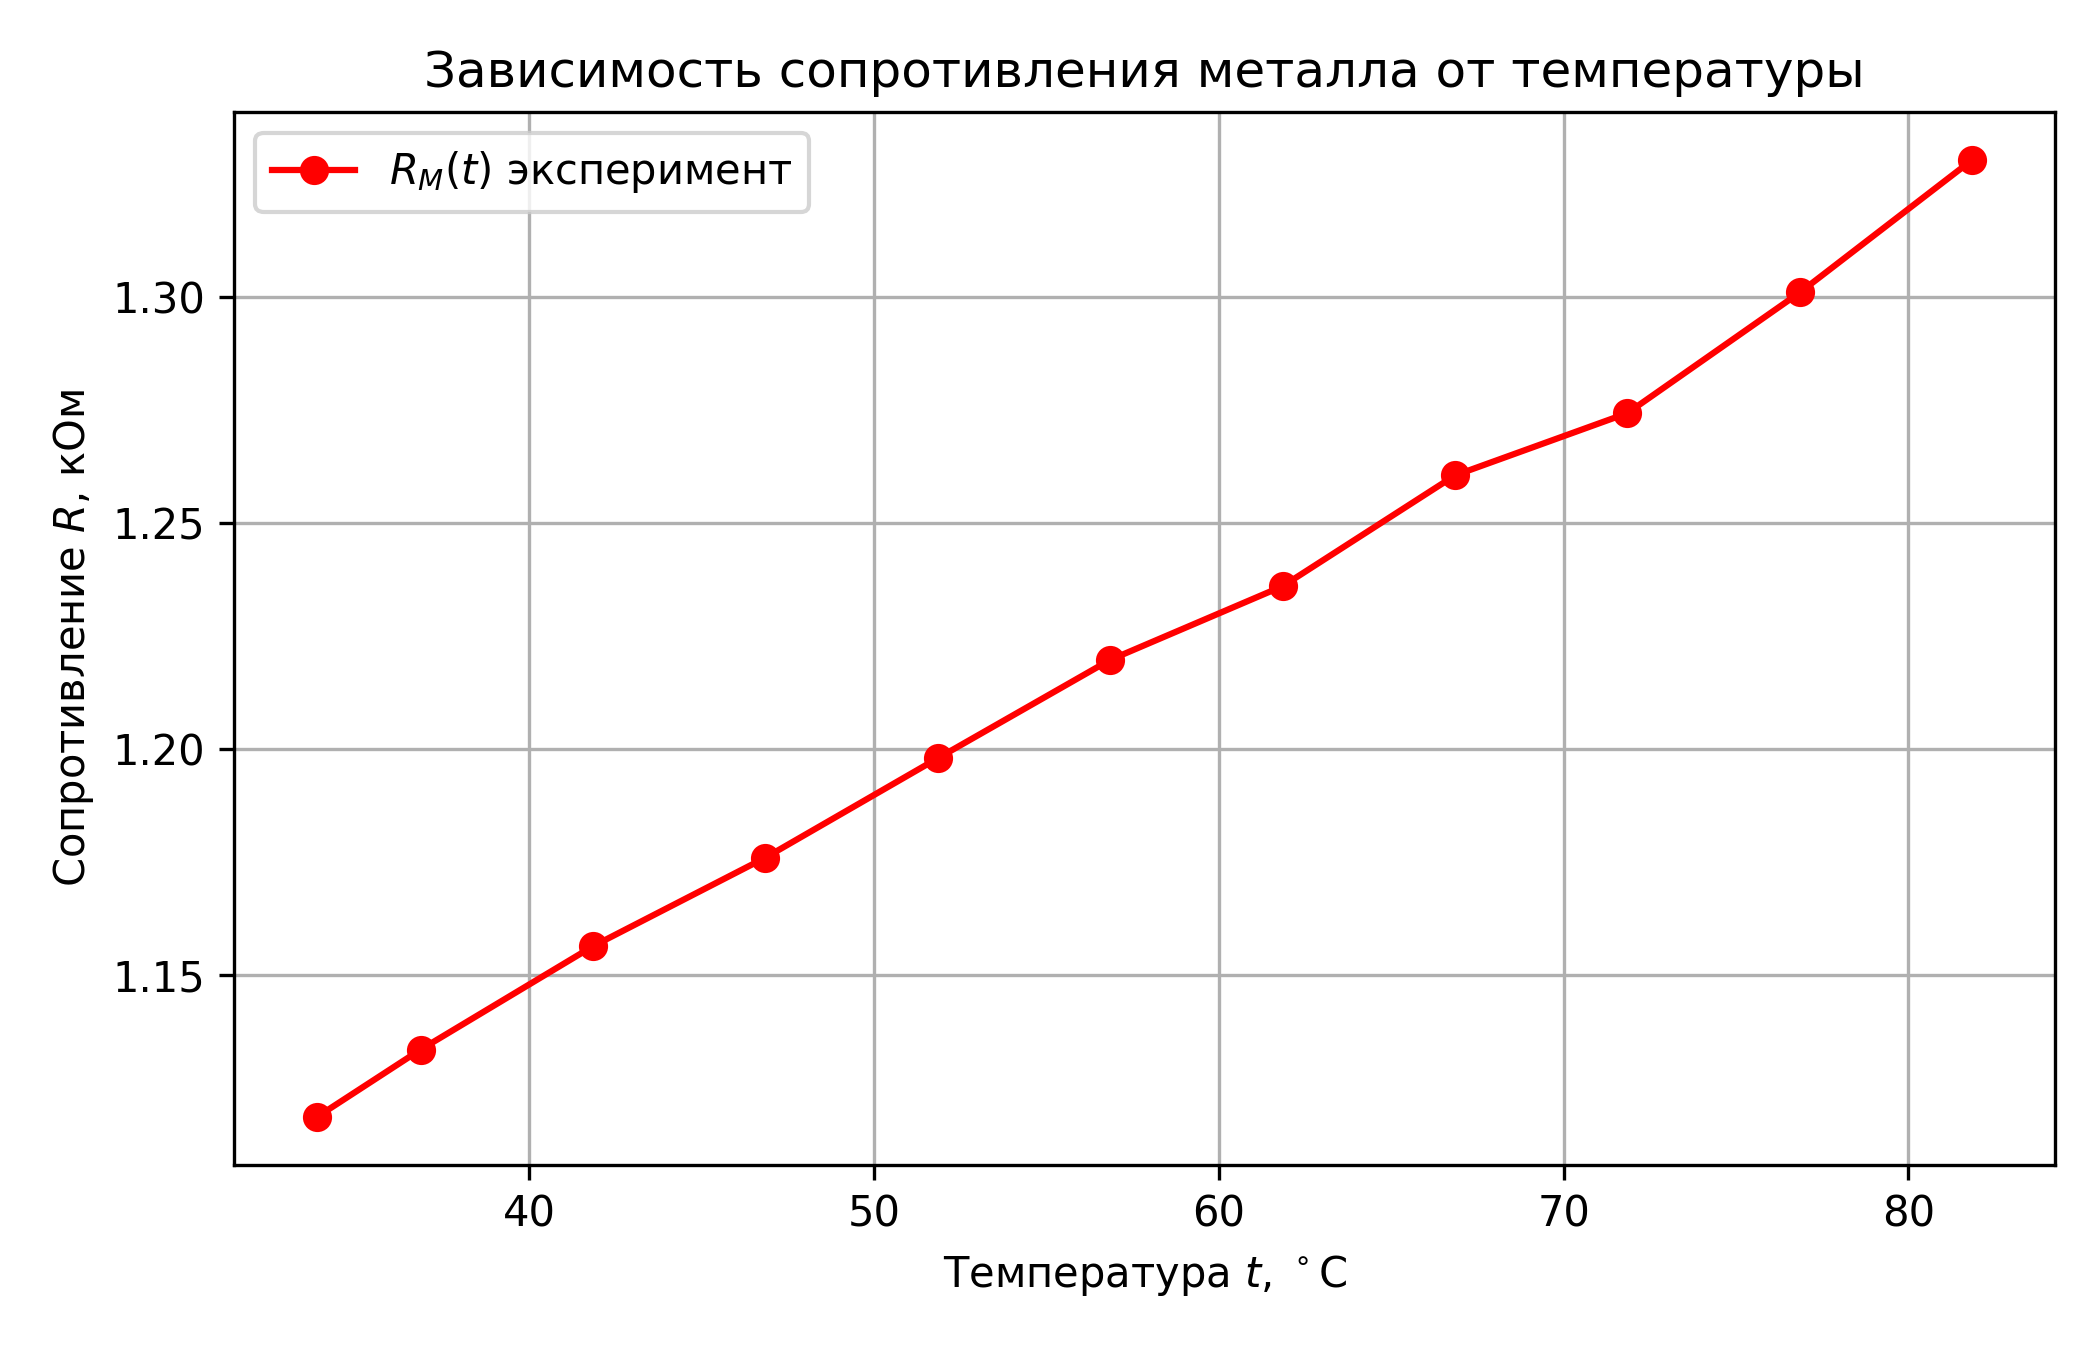
\includegraphics[width=0.75\textwidth]{metal_plot.png}
    \caption{Экспериментальный график зависимости сопротивления металла $R_M(t)$ от температуры}
    \label{fig:metal_plot}
\end{figure}

\begin{figure}[H]
    \centering
    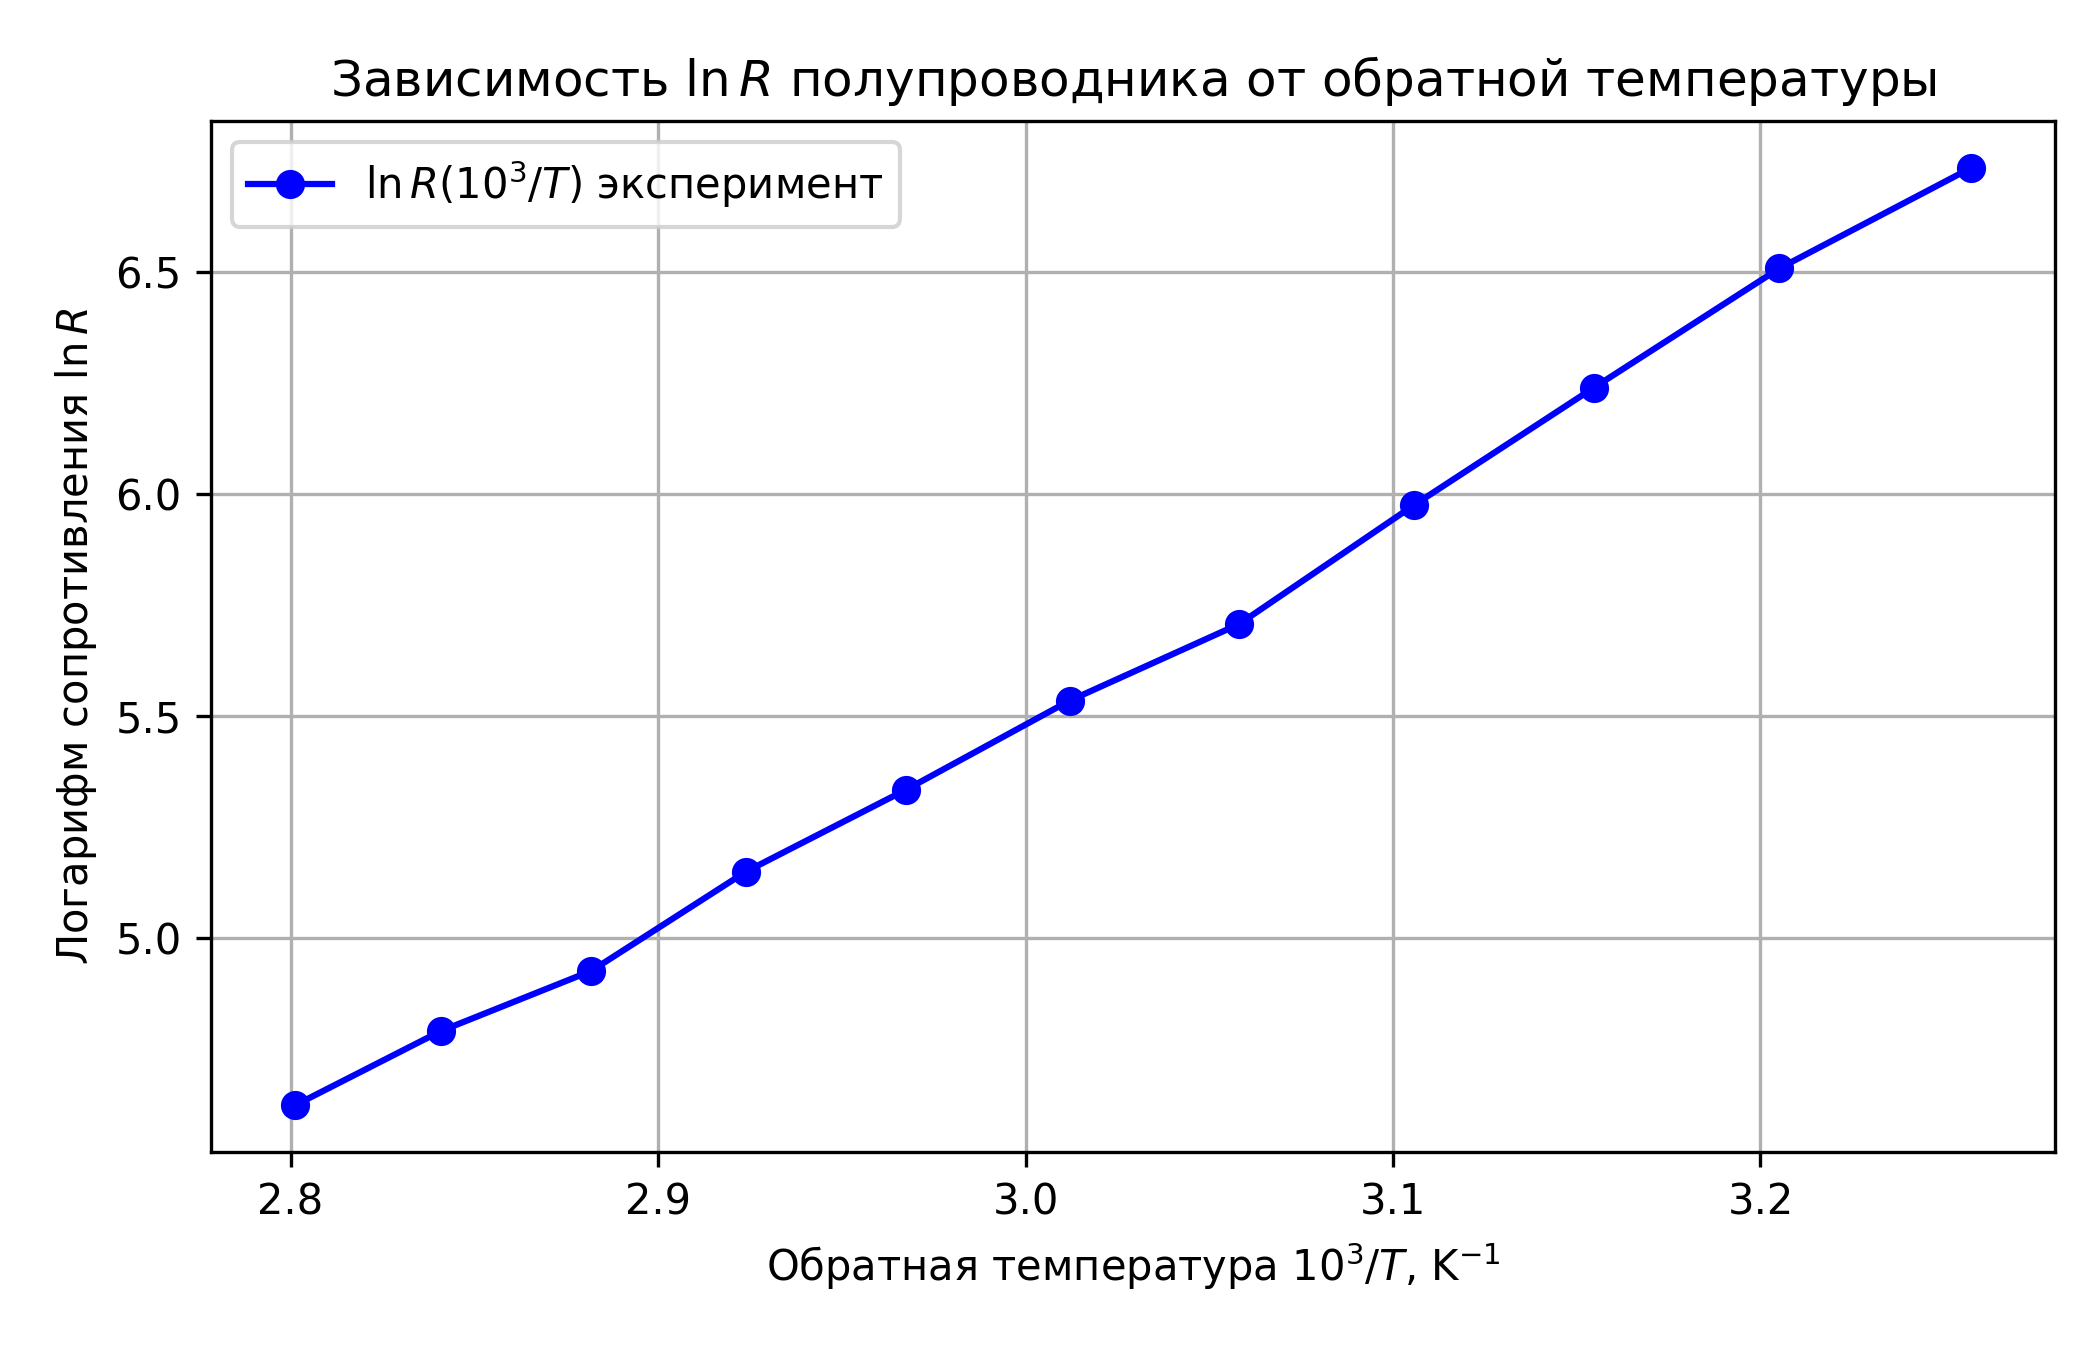
\includegraphics[width=0.75\textwidth]{semiconductor_plot.png}
    \caption{Экспериментальный график линеаризованной зависимости полупроводника $\ln(R / 1\,\text{Ом})$ от обратной температуры $10^3/T$}
    \label{fig:semi_plot}
\end{figure}

\newpage
\section{Выводы}
В ходе выполнения лабораторной работы экспериментально исследованы температурные зависимости электрического сопротивления металлического и полупроводникового образцов в температурном диапазоне от комнатной до $75~^{\circ}\text{C}$.

На основе полученных массивов данных аналитическим методом независимых пар точек были рассчитаны фундаментальные макроскопические характеристики материалов и проведен строгий метрологический анализ:
\begin{enumerate}
    \item Для металлического образца определен температурный коэффициент сопротивления $\alpha = (4{,}23 \pm 0{,}27) \cdot 10^{-3}~\text{К}^{-1}$ с относительной погрешностью $\varepsilon_\alpha = 6{,}4\%$. Чисто математически полученное значение ближе к справочному значению для чистого алюминия ($\alpha_{\text{справ}} = 4{,}20 \cdot 10^{-3}~\text{К}^{-1}$, относительное отклонение $\delta = 0{,}7\%$), нежели для чистой меди ($\alpha_{\text{справ}} = 4{,}30 \cdot 10^{-3}~\text{К}^{-1}$, отклонение $\delta = 1{,}6\%$). 
    Однако, опираясь на техническую документацию измерительного стенда «СЗ-ТТ01», исследуемый образец представляет собой медную проволочную катушку. Наблюдаемое экспериментальное занижение коэффициента $\alpha$ относительно чистой меди обусловлено влиянием комплекса систематических физических факторов: наличием естественных примесей в составе технической (а не химически чистой) меди, которые существенно снижают температурный коэффициент сопротивления, существованием температурного градиента между цифровым термодатчиком печи и внутренними слоями обмотки образца, а также неидеальностью контактных сопротивлений в измерительных цепях. Таким образом, с учетом данных факторов материал аргументированно идентифицирован как техническая медь.
    \item Для полупроводникового образца рассчитана ширина запрещенной зоны $E_g = 0{,}81 \pm 0{,}06~\text{эВ}$ ($(1{,}30 \pm 0{,}10) \cdot 10^{-19}~\text{Дж}$) с относительной погрешностью $\varepsilon_{E_g} = 7{,}4\%$. Экспериментальное значение указывает на то, что исследуемым материалом является \textbf{германий} ($Ge$). Наблюдаемое смещение относительно фундаментального теоретического значения чистой зоны для ультрачистого германия ($E_{g,\text{теор}} \approx 0{,}66{-}0{,}72~\text{эВ}$, отклонение от среднего значения $\delta \approx 14\%$) обусловлено физическими эффектами теплового сужения зоны при нагреве и донорным примесным легированием образца, используемого в лабораторных установках.
\end{enumerate}
Эксперимент наглядно подтвердил коренное различие двух механизмов проводимости: фононное рассеяние в металлах, ведущее к линейному росту сопротивления, и экспоненциальную тепловую активацию свободных носителей заряда в полупроводниках.

\newpage
\appendix
\section{Программный код для обработки данных}
В данном приложении приведен полный исходный код расчетного скрипта на языке Python, использованного для верификации вычислений и построения графиков.

\begin{lstlisting}[style=mypython, caption={Скрипт расчета параметров и графиков}]
import numpy as np
import matplotlib.pyplot as plt

# 1. Данные для полупроводникового образца
T_sem = np.array([307, 312, 317, 322, 327, 332, 337, 342, 347, 352, 357])
I_sem = np.array([1054, 1165, 1302, 1442, 1535, 1618, 1689, 1757, 1813, 1860, 1895]) # мкА
U_sem = np.array([0.886, 0.781, 0.667, 0.567, 0.462, 0.410, 0.350, 0.303, 0.250, 0.224, 0.193]) # В

R_sem = U_sem / (I_sem * 1e-6) # Ом
ln_R_sem = np.log(R_sem)
inv_T103 = 1000.0 / T_sem

# 2. Данные для металлического образца
T_met = np.array([355, 350, 345, 340, 335, 330, 325, 320, 315, 310, 307])
I_met = np.array([1026, 1043, 1057, 1063, 1076, 1083, 1096, 1108, 1119, 1131, 1138]) # мкА
U_met = np.array([1.365, 1.357, 1.347, 1.340, 1.330, 1.321, 1.313, 1.303, 1.294, 1.282, 1.273]) # В

R_met = (U_met / (I_met * 1e-6)) / 1000.0 # кОм
t_met = T_met - 273.15 # градусы Цельсия

print("Полупроводник R (Ом):", np.round(R_sem, 2))
print("Металл R (кОм):", np.round(R_met, 4))

# Построение графика для металла
plt.figure(figsize=(7, 4.5))
plt.plot(t_met, R_met, 'ro-', label='$R_M(t)$ эксперимент')
plt.xlabel(r'Температура $t$, $^\circ$C')
plt.ylabel('Сопротивление $R$, кОм')
plt.title('Зависимость сопротивления металла от температуры')
plt.grid(True)
plt.legend()
plt.tight_layout()
plt.savefig('metal_plot.png', dpi=300)
plt.close()

# Построение графика для полупроводника
plt.figure(figsize=(7, 4.5))
plt.plot(inv_T103, ln_R_sem, 'bo-', label=r'$\ln R(10^3/T)$ эксперимент')
plt.xlabel(r'Обратная температура $10^3/T$, K$^{-1}$')
plt.ylabel(r'Логарифм сопротивления $\ln R$')
plt.title(r'Зависимость $\ln R$ полупроводника от обратной температуры')
plt.grid(True)
plt.legend()
plt.tight_layout()
plt.savefig('semiconductor_plot.png', dpi=300)
plt.close()
\end{lstlisting}

\end{document}